\section{Strongly Coupled Dark Matter}\label{sec:darkqcd}

\subsection{Models}\label{subsec:models}

Dark QCD models include numerous parameters, with current searches focusing on those most immediately observable:
the mediator mass \mZprime or \mbifun, the dark hadron mass scale \mdark, and the invisible fraction \rinv.
The latter is the most novel parameter of the model, corresponding to the fraction of dark hadrons that are stable and invisible (DM candidates).
However, it is an effective parameter, summarizing the impacts of various accidental symmetries and conserved quantum numbers.
Many other dark sector parameters can impact the collider final state, including the cutoff scale \Lamdark, the dark quark mass \mqdark, the number of dark colors \Ncdark, and the number of dark flavors \Nfdark.
The details of the mediator connecting the SM and dark sector, such as its couplings, can affect the decays of unstable dark hadrons.
In addition, because low-energy QCD bound state formation via showering and hadronization is non-perturbative, it must be simulated using phenomenological models,
with parameters that are tuned to measurements of SM QCD.

The models currently investigated in CMS searches are based on Refs.~\cite{Cohen:2015toa,Cohen:2017pzm}, along with contributions from the PI
regarding the relationship between \mdark and \Lamdark, as well as the modeling of \rinv~\cite{Albouy:2022cin}.
These models choose $\Ncdark=2$ and $\Nfdark=2$, which leads to similarities in baryon and meson states that may not be modeled correctly,
given the lack of a confining $SU(2)$ force in the SM.
Here, we propose a more comprehensive assessment of the interplay between \Nfdark, \Lamdark, \mdark, and \mqdark (among other parameters),
focusing on the $\Ncdark=3$ case, for which lessons from the SM, especially from lattice QCD, can be more easily reused.
This will complete the original vision of the Snowmass effort, Ref.~\cite{Albouy:2022cin},
to deliver a complete set of benchmarks covering the entire range of \rinv values from 0 to 1,
reflecting new understanding about degeneracies in the model space and any nontrivial correlations between \rinv and observables such as jet substructure.
This new set of benchmarks can guide the Run 3 search strategy to ensure the entire known phase space is covered
and can serve to unify the efforts of different experimental collaborations, which currently study different models.

\subsection{Run 2 Searches}\label{subsec:run2}

% centered, fixed-width column type
\newcolumntype{C}[1]{w{c}{#1}}
\newlength\searchlen
\setlength\searchlen{.8cm}
\newlength\searchlena
\setlength\searchlena{2\searchlen}
\newlength\searchlenb
\setlength\searchlenb{3\searchlen}
\newlength\searchlenc
\setlength\searchlenc{6\searchlen}

\begin{figure}[htb!]
\begin{floatrow}
\ffigbox{%
\centering
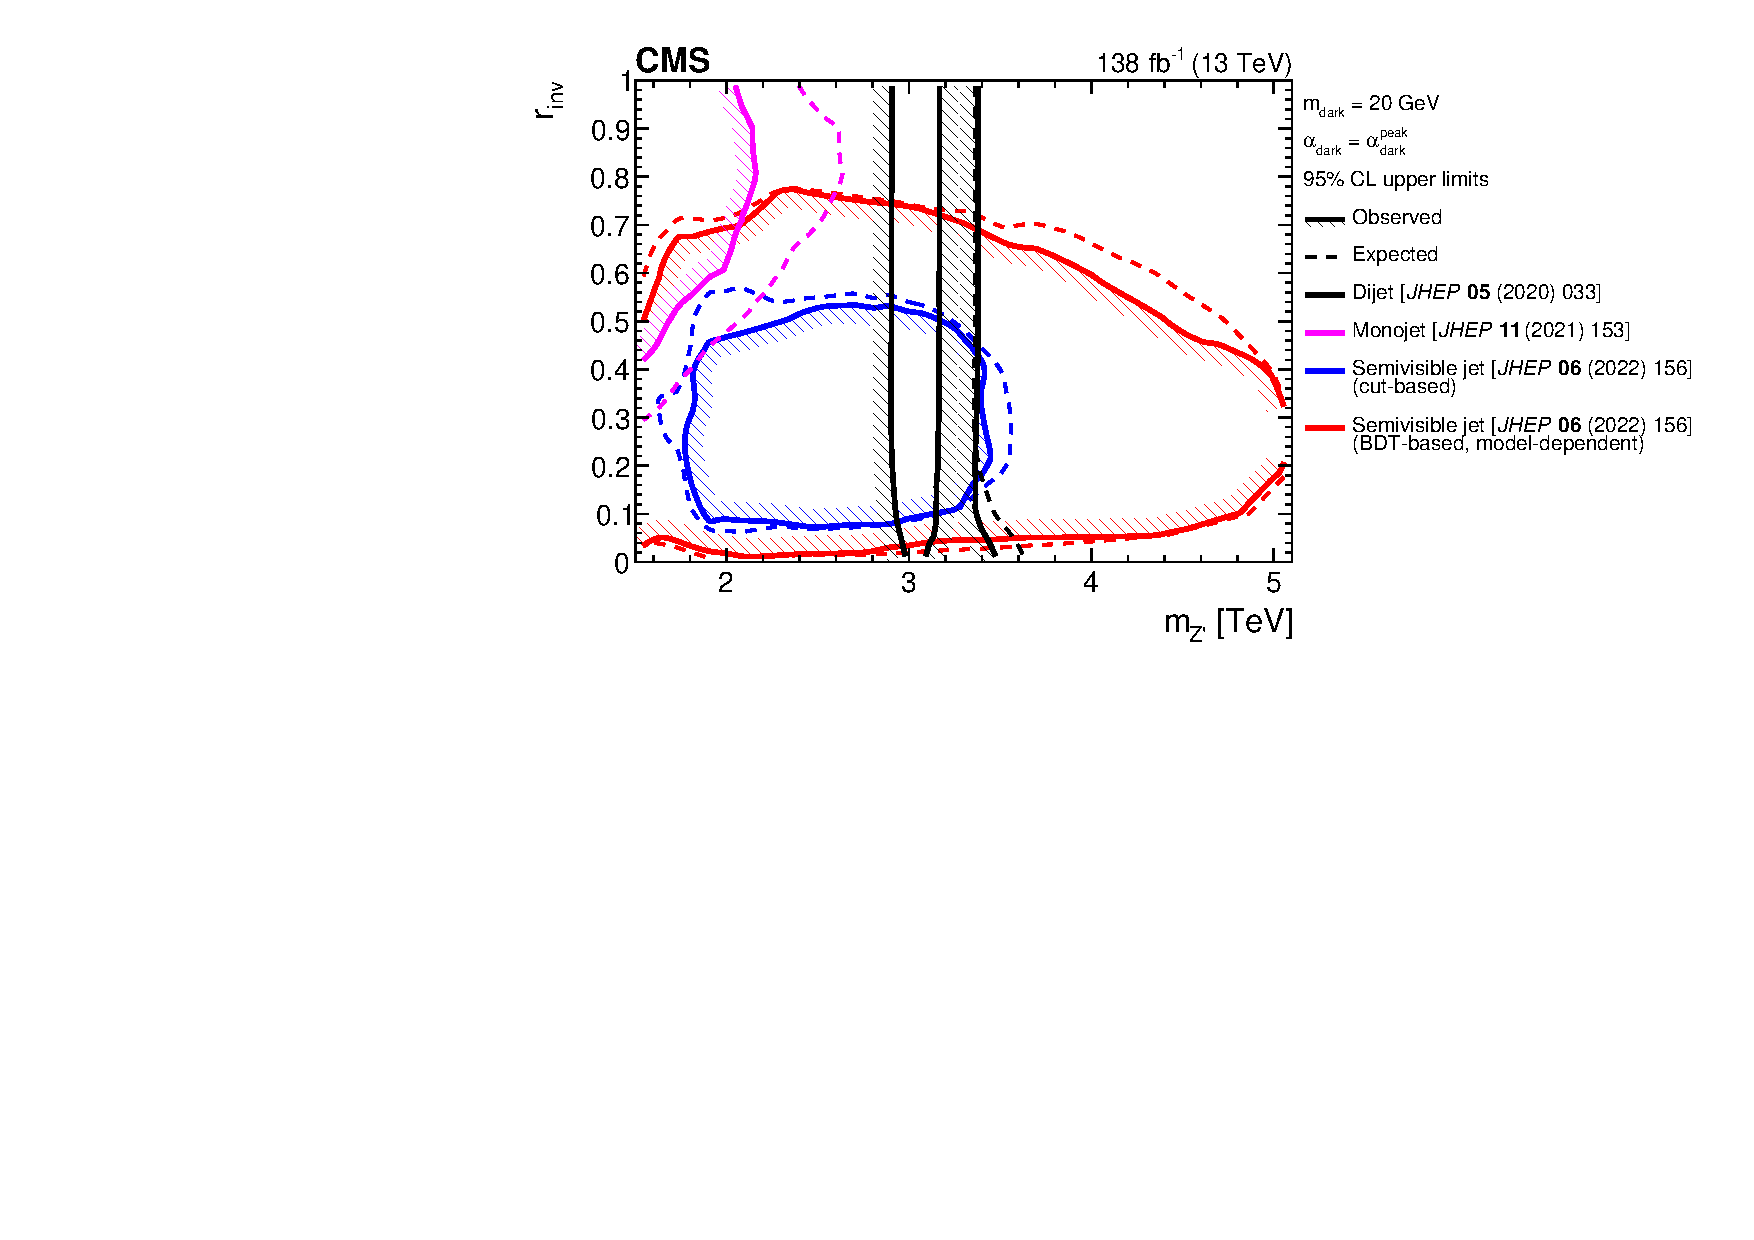
\includegraphics[width=0.49\textwidth]{figures/comp_limit_dijet_new_svj_monojet_2d.pdf}
}{\caption{Excluded regions of the \mZprime-\rinv plane from the SVJ search, dijet search, and monojet search.\label{fig:svjexcl}}}
\capbtabbox{%
\centering
\begin{tabular}{|c|*{6}{C{\searchlen}}|}
\hline
\multirow{2}{*}{Mediator} & \multicolumn{6}{C{\searchlenc}|}{Mass range} \\
& \multicolumn{2}{C{\searchlena}}{Low} & \multicolumn{2}{C{\searchlena}}{Medium} & \multicolumn{2}{C{\searchlena}|}{High} \\
\hline
\PZprime & \multicolumn{2}{C{\searchlena}}{\cellcolor{yellow!50}\makecell{standard\\(boosted)}} & \multicolumn{2}{C{\searchlena}}{\cellcolor{magenta!50}\makecell{scouting\\\vphantom{(boosted)}}} & \multicolumn{2}{C{\searchlena}|}{\cellcolor{orange!50}\makecell{standard\\\vphantom{(boosted)}}} \\
\hline
\Pbifun & \multicolumn{3}{C{\searchlenb}}{\cellcolor{orange!50}\makecell{standard\\\vphantom{(boosted)}}} & \multicolumn{3}{C{\searchlenb}|}{\cellcolor{magenta!50}\makecell{scouting\\\vphantom{(boosted)}}} \\
\hline
\end{tabular}
\vspace{\myfigureskip}
}{\caption{A summary of the conventional trigger options for different mediators and mass ranges for SVJ production.\label{tab:conventional}}}
\end{floatrow}
\end{figure}

The PI led the first search for semivisible jets, published in Ref.~\cite{CMS:2021dzg}, which targeted $s$-channel production via a massive \PZprime mediator.
This is the first dedicated analysis of collider events with jets aligned with missing transverse momentum,
a signature that usually arises in the SM via undermeasurement of a jet from a QCD multijet process.
This work built on the PI's previous leadership of searches for strongly-produced supersymmetric particles in hadronic final states~\cite{Khachatryan:2016kdk,Sirunyan:2017cwe,Sirunyan:2019hzr,Sirunyan:2019ctn,CMS:2023xlp}.
The search also introduced the dual strategy of providing both model-independent and model-dependent results,
with the latter utilizing a boosted decision tree (BDT) trained to identify SVJs from specific signal models using high-level variables focusing on jet substructure.
Figure~\ref{fig:svjexcl} compares the mass and coupling exclusions from this search to the dijet resonance search, which targets the complementary process $\PZprime \to \cPq\cPaq$,
and the monojet search, which targets a signature of simplified DM models, \ptmiss in association with an initial-state radiation (ISR) jet.
Even the simple cut-based model-independent strategy offers a noticeable improvement over other searches in the area around $\rinv=0.3$, where the acceptance is maximized.

Subsequently, the PI has developed several more searches, now nearing completion, that use the LHC Run 2 dataset to target different mass ranges and production modes:
low-mass \PZprime, intermediate-mass \PZprime, and nonresonant $t$-channel production through a bifundamental scalar mediator \Pbifun,
which has Yukawa couplings \sbifun between SM quarks and dark quarks~\cite{Cohen:2017pzm}.
Each search requires a different trigger strategy, summarized in Table~\ref{tab:conventional}.
These include conventional triggers based on jet \pt, \HT (the scalar sum of jet \pt), and \ptmiss;
triggering on ISR jet \pt in a boosted topology;
and the use of data scouting, in which a lower threshold in the \HT trigger is enabled by storing only partial event information~\cite{Mukherjee:2019anz}.

\subsection{Run 3 Strategy}\label{subsec:strategy}

We propose a new, unified trigger strategy in Run 3, made possible by the introduction of anomaly detection triggers based on unsupervised AI.
Two complementary algorithms are available: CICADA~\cite{CMS-DP-2023-086}, which looks for anomalous calorimeter clusters, and AXOL1TL~\cite{CMS-DP-2023-079}, which looks for global anomalies.
These algorithms are developed by the PI's Fermilab, CERN, and LPC colleagues, and the PI has been involved with validating and improving the performance of these triggers on dark QCD models;
the latest results are shown in Fig.~\ref{fig:svjanomaly}.
The anomaly triggers promise substantial improvements in the signal trigger efficiency, especially for lower-mass \PZprime mediators and nonresonant production,
which will facilitate sensitivity to more models and smaller couplings.

\begin{figure}[htb!]
\centering
\twofigeqh{figures/axol1tl_score_schan.pdf}{figures/axol1tl_score_tchan2.pdf}
\caption{Score distributions from anomaly triggers on SVJ processes. (PLACEHOLDER)}
\label{fig:svjanomaly}
\end{figure}

We will further unify the offline analysis strategy to cover all production modes.
Currently, no search targets resonant production of \Pbifun, which is more prominent for low mediator mass and small \sbifun, and can occur singly in association with a low-\pt SVJ, or in a pair.
The PI has demonstrated that a form of semi-supervised, interpretable AI called the event variable network (EVN)
can learn optimal mass reconstruction functions, superseding the standard transverse mass and similar variables~\cite{Pedro:2023sdp}.
Figure~\ref{fig:svjmass} (left) shows an example result for \Pbifun pair production; other studies show that the EVN is robust against signal model parameter variations.
We will extend this concept to a jet variable network (JVN) by incorporating a graph neural network (GNN) to look inside the jets.
This new approach is inspired by the observations from Refs.~\cite{Strassler:2008fv,CMS:2021dzg} that conventional subjet or jet grooming techniques, when applied to SVJs, reflect the dark hadron mass scale \mdark.
This is shown in Fig.~\ref{fig:svjmass} (right) for the soft drop algorithm~\cite{Larkoski:2014wba}, which captures the \mdark when there is a single hard fragmentation during the showering process.
The JVN will extract \mdark more efficiently by implicitly reconstructing the originating dark hadrons.
By searching in the distribution of the JVN output, a per-jet variable, we will achieve sensitivity to SVJs regardless of the production mode.

\begin{figure}[htb!]
\centering
\twofigeqh{figures/signif_tchanPair.pdf}{figures/EXO-19-020_Figure_003-a.pdf}
\caption{Left: The distributions of the classical (\mTii) and learned ($V$) mass variables for \Pbifun pair production and QCD background; the middle pane shows the significance, and the bottom pane shows the significance improvement. Right: The softdrop mass distributions for SVJs with different \mdark values and SM backgrounds, normalized to unit area.}
\label{fig:svjmass}
\end{figure}

\subsection{SVJ Tagging}\label{subsec:tagging}

The identification or ``tagging'' of SVJs is another critical element, as this is the only way to reduce the large SM backgrounds beyond basic event-level kinematic selections.
From the original BDT, the team has progressed to more sophisticated approaches:
a supervised (model-dependent) tagger using particle-level inputs, based on the ParticleNet GNN architecture~\cite{Qu:2019gqs};
and an unsupervised (model-independent) autoencoder (AE) using jet substructure variables.
The current performance of these algorithms is shown in Fig.~\ref{fig:svjtaggers}, quantified by integrating the receiver-operator characteristic (ROC) curve to produce the area under the curve (AUC).
A comparable ParticleNet-based supervised tagger for EMJs has AUC scores of 0.97--0.99, indicating that it is markedly more difficult to distinguish SVJs from QCD jets.

\begin{figure}[htb!]
\centering
\twofigeqh{figures/rocScoreSigP2DQCD_rinv.pdf}{figures/WNAE_performance_from_SVJ_t_channel_status_update_2024_02_06-2.pdf}
\caption{The AUC performance of the latest SVJ taggers: supervised ParticleNet (left) and unsupervised Wasserstein normalized autoencoder (right).
A score of 1.0 would indicate perfect discrimination between signal and background jets.}
\label{fig:svjtaggers}
\end{figure}

The AE only learns to reconstruct common SM background processes and therefore discriminates against other processes by failing to reconstruct their kinematic features.
The PI was among the first to demonstrate the autoencoders could discriminate between SM QCD jets and SVJs, even surpassing a supervised tagger when applied to a signal model not used during training~\cite{Canelli:2021aps}.
To achieve discrimination against \ttbar jets, the normalized autoencoder (NAE) formalism~\cite{Dillon:2022mkq} was adopted in order to minimize complexity bias.
The team developed a completely novel method to stabilize the training by directly minimizing the Wasserstein or earth mover's distance
between samples drawn from the input data and from the latent representation of the autoencoder, resulting in the WNAE~\cite{Eble:2024tpr}.
This approach is also being applied to improve the AXOL1TL anomaly trigger.

For the Run 3 SVJ search, we will develop a new tagger combining the best features of both approaches:
a GNN-based autoencoder (GAE), using the Lund plane representation following Ref.~\cite{Dreyer:2020brq} and trained with the WNAE approach.
Early attempts indicate the WNGAE could approach the performance level of the supervised tagger, while remaining naturally model-independent.
While these taggers are initially trained using simulated events,
the semi-supervised universal domain adaptation technique developed by the PI and his collaborators~\cite{Ciprijanovic:2023hrw}
will be employed to ensure similar performance in data by learning only physically invariant features.

\subsection{Dark QCD Scan}\label{subsec:darkscan}

While this proposal focuses on SVJs, there are other dark QCD phenomena.
EMJs may form if the unstable dark hadrons have a lifetime \taudark, leading to multiple displaced vertices within a single jet.
SUEPs occur when there is a large 't Hooft coupling strength $\thooft = \gdark^2 \Ncdark$,
resulting in a high multiplicity of low-momentum tracks from unsuppressed large angle emissions, rather than collimated jets.
The CMS Dark QCD team has recently released new results for both signatures in Refs.~\cite{CMS:2023vpb,CMS:2024emj},
following the first CMS EMJ search with a small dataset~\cite{Sirunyan:2018njd}.
Conducting separate searches for each phenomenon is important to understand the kinematic phase space and behavior associated with these new models.

\begin{figure}[bht]
\centering
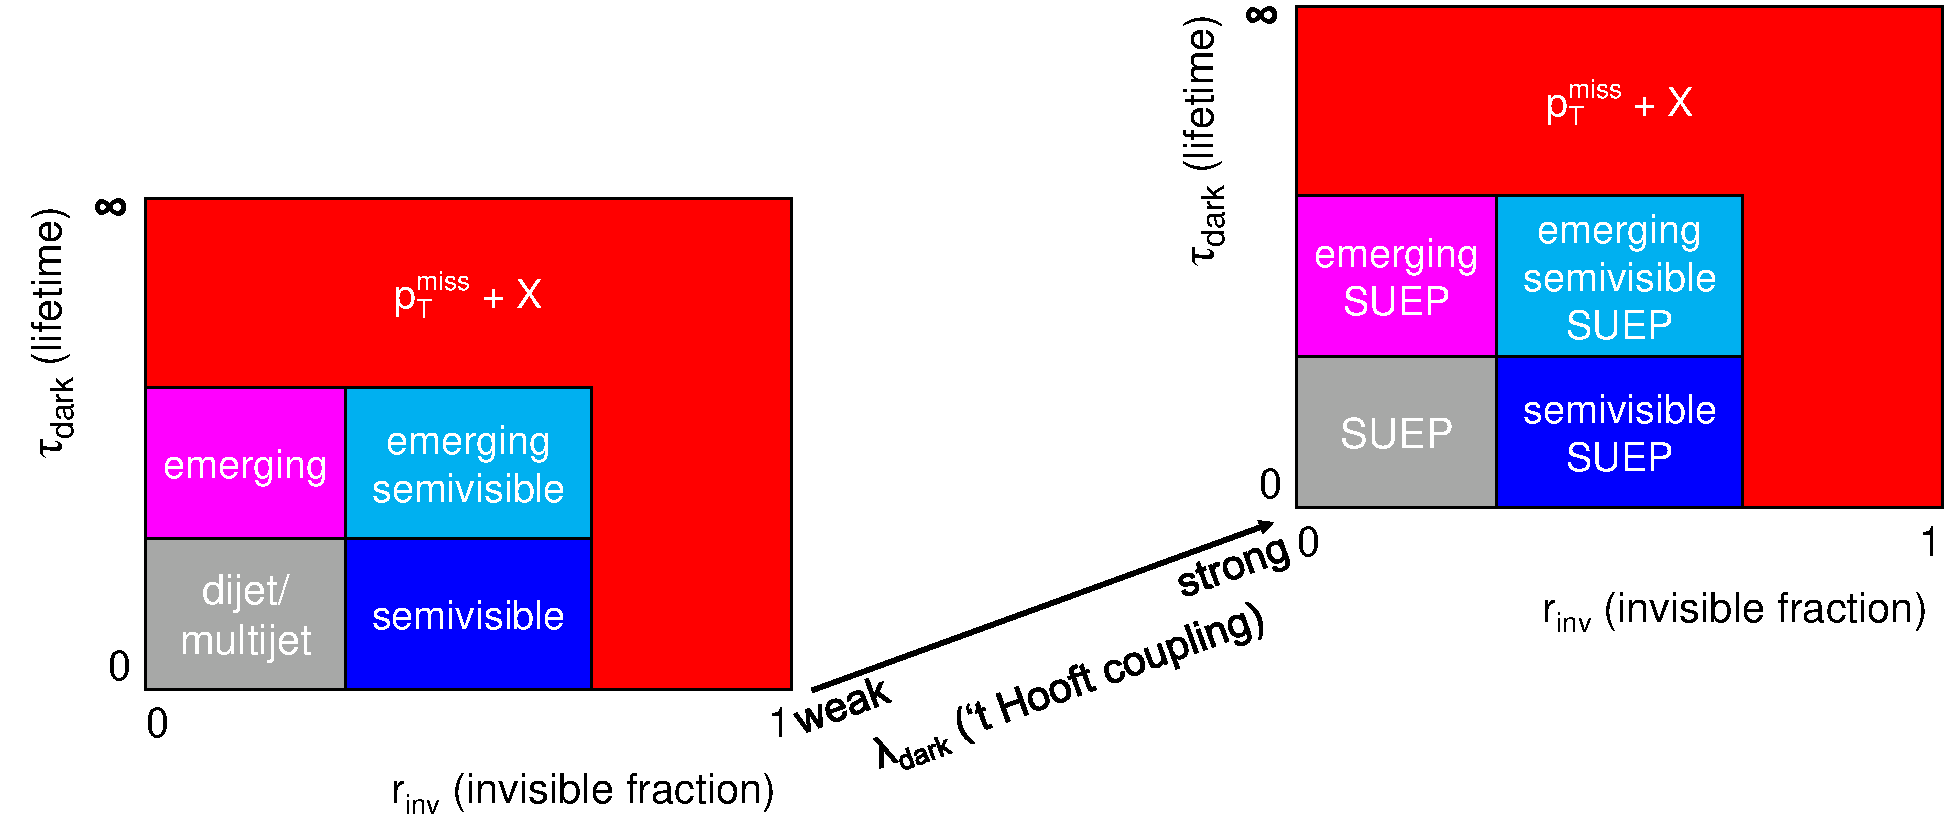
\includegraphics[width=0.95\myfigurewidth]{figures/svj_acceptance_diagram_v7.pdf}
\caption{A diagram illustrating the phenomena and search strategies with maximal acceptance for different combinations of dark QCD parameters.}
\label{fig:svjacc}
\end{figure}

However, it is not required, or even necessarily likely, that each of these phenomena should appear in isolation.
It is entirely possible that nature could produce semivisible emerging SUEPs or any other combination.
Figure~\ref{fig:svjacc} illustrates the interplay between three characteristic parameters:
the dark meson lifetime $\taudark$, the invisible fraction $\rinv$, and the 't Hooft coupling \thooft.
For large values of \rinv and \taudark, the pre-existing searches for large \met would still be the most effective.
However, for intermediate values of those parameters, a dedicated strategy might outperform any of the individual searches noted above.
The best strategies for large values of \thooft in combination with the other parameters remain an open question,
while the generation of physically realistic events at intermediate \thooft has only recently become possible~\cite{Cesarotti:2020uod}.

All of these search strategies might need adjustments for other parameter variations,
such as the mediator masses and couplings and the various dark sector parameters discussed in Section~\ref{subsec:models}.
The most feasible way to explore this large parameter space is using a multidimensional scan,
similar to scans of the phenomenological minimal supersymmetric standard model (pMSSM)~\cite{Djouadi:1998di}
provided by CMS for earlier datasets~\cite{Khachatryan:2016nvf,SUS-16-033-supp} and currently in preparation for Run 2 by the PI and his colleagues.
Much like the pMSSM, this scan will include many random parameter combinations, with existing constraints included to eliminate models that are already ruled out.
We will reinterpret the latest dark QCD searches from LHC Runs 2 and 3 to understand which of these combined models are effectively excluded and which are not covered.
Finding uncovered models will direct efforts to design new search strategies, including dedicated triggers, for the upcoming HL-LHC runs.
The combined models will also help to further characterize any observed signal, which would likely have intermediate values of some parameters.

Obtaining the strongest results from the dark QCD scan relies on the success of the Run 3 SVJ search.
The proposed strategy includes several new elements, any of which may not converge on the necessary timescale.
However, each new element is independent from the others, and reasonable fallback options exist to mitigate these risks:
\begin{enumerate}
\item \textit{Model building}: if a comprehensive set of new benchmarks is not available, the existing models can be used, at the cost of potentially reduced coverage of the model space.
\item \textit{Anomaly triggers}: if the anomaly trigger performance is not sufficient, the Run 2 trigger strategy can be used, at the cost of more effort to analyze multiple datasets with a less unified strategy.
\item \textit{Jet variable network}: if the JVN does not perform as expected or is not sufficiently model-independent, we will consider classical techniques such as the softdrop algorithm, at the cost of reduced efficiency. Alternatively, we will fall back to the event-level strategy, still using the optimal mass variables learned by the EVN along with \ptmiss in the nonresonant case, at the cost of additional effort and dependence on production mode.
Even then, a common background estimation technique will be employed, utilizing the new ``closure loss'' developed by the PI and his colleagues
to optimize a neural network to perform an ``ABCD'' background estimation using three control regions in observed data~\cite{Crossman:2023aps}.
\item \textit{SVJ taggers}: if the WNGAE encounters difficulties, the existing tagger architectures can be reused, at the cost of decreased tagging performance or increased model dependence. (The same applies to other AI algorithms, which can be substituted with standard techniques at the cost of increased uncertainty or decreased sensitivity.)
\end{enumerate}
At minimum, the SVJ search will benefit from the use of the larger, higher energy Run 3 dataset.
Current searches do not exclude a \PZprime of mass 6\TeV, or alternatively pair production of \Pbifun with mass 3\TeV;
the discovery significance for these models will increase by a factor of 2.0--2.4.
This higher mass reach is driven primarily by the 80\% higher production cross section at $\sqrt{s}=13.6\TeV$ compared to 13\TeV;
access to weaker processes with smaller coupling values, at all masses, will improve with the integrated luminosity of ${\sim}$190--260\fbinv compared to 138\fbinv.
Given these risk mitigation strategies, we expect strong results from this search program.
